\documentclass[14pt]{extbook}
\usepackage{multicol, enumerate, enumitem, hyperref, color, soul, setspace, parskip, fancyhdr} %General Packages
\usepackage{amssymb, amsthm, amsmath, bbm, latexsym, units, mathtools} %Math Packages
\everymath{\displaystyle} %All math in Display Style
% Packages with additional options
\usepackage[headsep=0.5cm,headheight=12pt, left=1 in,right= 1 in,top= 1 in,bottom= 1 in]{geometry}
\usepackage[usenames,dvipsnames]{xcolor}
\usepackage{dashrule}  % Package to use the command below to create lines between items
\newcommand{\litem}[1]{\item#1\hspace*{-1cm}\rule{\textwidth}{0.4pt}}
\pagestyle{fancy}
\lhead{Progress Quiz 4}
\chead{}
\rhead{Version A}
\lfoot{9187-5854}
\cfoot{}
\rfoot{Spring 2021}
\begin{document}

\begin{enumerate}
\litem{
Find the equation of the line described below. Write the linear equation as $ y=mx+b $ and choose the intervals that contain $m$ and $b$.\[ \text{Parallel to } 9 x - 5 y = 14 \text{ and passing through the point } (-2, -4). \]\begin{enumerate}[label=\Alph*.]
\item \( m \in [1.4, 2.1] \hspace*{3mm} b \in [-2.97, -1.69] \)
\item \( m \in [-2.9, -0.8] \hspace*{3mm} b \in [-8.65, -6.65] \)
\item \( m \in [0.3, 1.1] \hspace*{3mm} b \in [-0.69, 0.25] \)
\item \( m \in [1.4, 2.1] \hspace*{3mm} b \in [-0.69, 0.25] \)
\item \( m \in [1.4, 2.1] \hspace*{3mm} b \in [0.17, 1.08] \)

\end{enumerate} }
\litem{
First, find the equation of the line containing the two points below. Then, write the equation as $ y=mx+b $ and choose the intervals that contain $m$ and $b$.\[ (4, -10) \text{ and } (8, 5) \]\begin{enumerate}[label=\Alph*.]
\item \( m \in [0.75, 7.75] \hspace*{3mm} b \in [-5, 3] \)
\item \( m \in [0.75, 7.75] \hspace*{3mm} b \in [19, 31] \)
\item \( m \in [-3.75, -2.75] \hspace*{3mm} b \in [34, 36] \)
\item \( m \in [0.75, 7.75] \hspace*{3mm} b \in [-26, -21] \)
\item \( m \in [0.75, 7.75] \hspace*{3mm} b \in [-15, -13] \)

\end{enumerate} }
\litem{
Find the equation of the line described below. Write the linear equation as $ y=mx+b $ and choose the intervals that contain $m$ and $b$.\[ \text{Parallel to } 3 x + 5 y = 15 \text{ and passing through the point } (10, 3). \]\begin{enumerate}[label=\Alph*.]
\item \( m \in [-0.91, -0.12] \hspace*{3mm} b \in [-8.7, -6.3] \)
\item \( m \in [-0.91, -0.12] \hspace*{3mm} b \in [-11.6, -8.1] \)
\item \( m \in [-0.91, -0.12] \hspace*{3mm} b \in [8.8, 9.2] \)
\item \( m \in [-1.72, -0.61] \hspace*{3mm} b \in [8.8, 9.2] \)
\item \( m \in [0.26, 1.97] \hspace*{3mm} b \in [-3.4, -2.1] \)

\end{enumerate} }
\litem{
Write the equation of the line in the graph below in Standard form $Ax+By=C$. Then, choose the intervals that contain $A, B, \text{ and } C$.
\begin{center}
    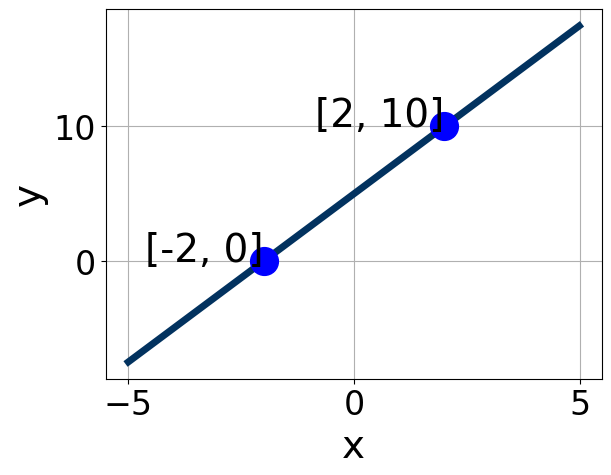
\includegraphics[width=0.5\textwidth]{../Figures/linearGraphToStandardCopyA.png}
\end{center}
\begin{enumerate}[label=\Alph*.]
\item \( A \in [-5.1, -4.2], \hspace{3mm} B \in [1.65, 2.49], \text{ and } \hspace{3mm} C \in [10, 12] \)
\item \( A \in [3.9, 7.3], \hspace{3mm} B \in [1.65, 2.49], \text{ and } \hspace{3mm} C \in [10, 12] \)
\item \( A \in [-3.1, -0.2], \hspace{3mm} B \in [0.93, 1.23], \text{ and } \hspace{3mm} C \in [1, 6] \)
\item \( A \in [3.9, 7.3], \hspace{3mm} B \in [-2.14, -1.8], \text{ and } \hspace{3mm} C \in [-11, -6] \)
\item \( A \in [-3.1, -0.2], \hspace{3mm} B \in [-1.38, -0.9], \text{ and } \hspace{3mm} C \in [-8, -3] \)

\end{enumerate} }
\litem{
Write the equation of the line in the graph below in Standard form $Ax+By=C$. Then, choose the intervals that contain $A, B, \text{ and } C$.
\begin{center}
    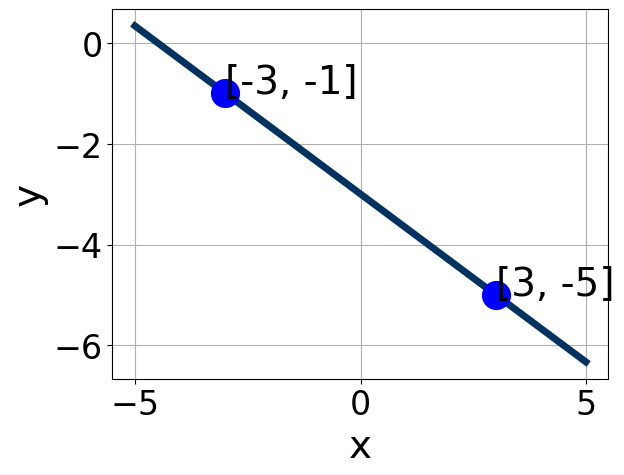
\includegraphics[width=0.5\textwidth]{../Figures/linearGraphToStandardA.png}
\end{center}
\begin{enumerate}[label=\Alph*.]
\item \( A \in [-1.25, 0.75], \hspace{3mm} B \in [-3.9, -0.6], \text{ and } \hspace{3mm} C \in [-3, 1] \)
\item \( A \in [-1.25, 0.75], \hspace{3mm} B \in [0, 3.3], \text{ and } \hspace{3mm} C \in [1, 6] \)
\item \( A \in [3, 7], \hspace{3mm} B \in [-5.5, -3], \text{ and } \hspace{3mm} C \in [-14, -7] \)
\item \( A \in [-13, -4], \hspace{3mm} B \in [1.5, 6.4], \text{ and } \hspace{3mm} C \in [4, 13] \)
\item \( A \in [3, 7], \hspace{3mm} B \in [1.5, 6.4], \text{ and } \hspace{3mm} C \in [4, 13] \)

\end{enumerate} }
\litem{
Solve the equation below. Then, choose the interval that contains the solution.\[ -8(18x -11) = -2(-10x + 15) \]\begin{enumerate}[label=\Alph*.]
\item \( x \in [0.43, 0.57] \)
\item \( x \in [0.69, 0.81] \)
\item \( x \in [-0.44, -0.24] \)
\item \( x \in [0.33, 0.45] \)
\item \( \text{There are no real solutions.} \)

\end{enumerate} }
\litem{
Solve the linear equation below. Then, choose the interval that contains the solution.\[ \frac{5x -3}{8} - \frac{7x + 9}{2} = \frac{-9x + 8}{4} \]\begin{enumerate}[label=\Alph*.]
\item \( x \in [0.3, 1] \)
\item \( x \in [-11.4, -10] \)
\item \( x \in [-33.1, -30.2] \)
\item \( x \in [2.4, 4.3] \)
\item \( \text{There are no real solutions.} \)

\end{enumerate} }
\litem{
Solve the equation below. Then, choose the interval that contains the solution.\[ -12(19x + 17) = -16(-11x -4) \]\begin{enumerate}[label=\Alph*.]
\item \( x \in [-0.76, -0.4] \)
\item \( x \in [-0.32, 0.56] \)
\item \( x \in [-2.89, -1.82] \)
\item \( x \in [-0.47, -0.29] \)
\item \( \text{There are no real solutions.} \)

\end{enumerate} }
\litem{
Solve the linear equation below. Then, choose the interval that contains the solution.\[ \frac{4x -5}{6} - \frac{7x + 7}{3} = \frac{-7x -3}{4} \]\begin{enumerate}[label=\Alph*.]
\item \( x \in [-30, -26] \)
\item \( x \in [-2.4, 4.6] \)
\item \( x \in [108, 110] \)
\item \( x \in [29, 32] \)
\item \( \text{There are no real solutions.} \)

\end{enumerate} }
\litem{
First, find the equation of the line containing the two points below. Then, write the equation as $ y=mx+b $ and choose the intervals that contain $m$ and $b$.\[ (-3, 4) \text{ and } (4, -8) \]\begin{enumerate}[label=\Alph*.]
\item \( m \in [-3, -0.6] \hspace*{3mm} b \in [0.6, 4.3] \)
\item \( m \in [-3, -0.6] \hspace*{3mm} b \in [-1.7, 1] \)
\item \( m \in [-3, -0.6] \hspace*{3mm} b \in [-13.3, -9.7] \)
\item \( m \in [-3, -0.6] \hspace*{3mm} b \in [6.2, 8.9] \)
\item \( m \in [0, 3.2] \hspace*{3mm} b \in [-15.1, -14.8] \)

\end{enumerate} }
\end{enumerate}

\end{document}